% !TEX root =../ECE343_Slides_Rogers.tex

%\begin{comment}
\section{Schedule}
\renewcommand{\arraystretch}{1}
\begin{frame}{}
	\begin{textblock}{14}(0.5,1.75)
	\def\myfontsize{footnotesize}
	
\setcounter{mylnum}{1}
\begin{center}
\begin{\myfontsize}
\begin{tabular}{| c | l | c | l |}
\hline
\textbf{Lesson} 		  	& \textbf{Topics}             & \pbox{5cm}{\textbf{Reading}}	& \textbf{Notes}		\\ \hline\hline
\ifnum\lessonNum=\value{mylnum} \rowcolor{green!20!white}\fi
	\themylnum  
	& Course Overview  \& Introduction		
	& Ch.1 
	&  LO 1.1-1.2 
	\stepcounter{mylnum}\\ \hline \hline
\rowcolor{gray!20!white}\multicolumn{4}{| c |}{\textbf{Chapter 2: Electric and Magnetic Fields}}	\\ \hline\hline
\ifnum\lessonNum=\value{mylnum} \rowcolor{green!20!white}\fi
	\themylnum 	
	& Fields, Parameters, Field Quantities	
	& Ch. 2	
	& LO 2.1-2.2			
\stepcounter{mylnum}\\ \hline\hline
\rowcolor{gray!20!white}\multicolumn{4}{| c |}{\textbf{Chapter 3: Transmission Lines}}	 \\ \hline\hline	
\ifnum\lessonNum=\value{mylnum} \rowcolor{green!20!white}\fi
	\themylnum 	
	& Lumped Element Model				
	& 3.1-3.4 
	& LO 3.1		
\stepcounter{mylnum}\\ \hline
\ifnum\lessonNum=\value{mylnum} \rowcolor{green!20!white}\fi
	\themylnum 	
	& Telegrapher's Equations
	& 3.5-3.6
	&  LO 3.1	
\stepcounter{mylnum}\\ \hline
\ifnum\lessonNum=\value{mylnum} \rowcolor{green!20!white}\fi
	\themylnum 	
	&  Characteristic Impedance \& Wave Propagation	
	& 3.7-3.9		
	& LO 3.2						
\stepcounter{mylnum}\\ \hline
\ifnum\lessonNum=\value{mylnum} \rowcolor{green!20!white}\fi
	\themylnum 	
	& Coaxial,  Reflection Coefficient, VSWR	
	& 3.10,3.12-3.14	
	& LO 3.2-3.3		
\stepcounter{mylnum}\\ \hline 
\ifnum\lessonNum=\value{mylnum} \rowcolor{green!20!white}\fi
	\themylnum 	
	&  Terminated Transmission Lines	
	&  3.15,3.17-3.19
	& LO 3.4		
\stepcounter{mylnum}\\ \hline 
\ifnum\lessonNum=\value{mylnum} \rowcolor{green!20!white}\fi
	\themylnum	
	& Impedance Matching	
	& 3.21-3.23
	& LO 3.4 			
\stepcounter{mylnum}\\ \hline 
\ifnum\lessonNum=\value{mylnum} \rowcolor{green!20!white}\fi
	\themylnum  
	& Impedance Matching	
	& 3.21-3.23
	& LO 3.4		
\stepcounter{mylnum}\\ \hline 
\ifnum\lessonNum=\value{mylnum} \rowcolor{green!20!white}\fi
	\themylnum	
	& Smith Charts
	& Supplemental
	& LO 3.5
\stepcounter{mylnum}\\ \hline 
\ifnum\lessonNum=\value{mylnum} \rowcolor{green!20!white}\fi
	\themylnum	
	& Smith Charts
	& Supplemental 
	& LO 3.5					
\stepcounter{mylnum}\\ \hline 
\ifnum\lessonNum=\value{mylnum} \rowcolor{green!20!white}\fi
	\themylnum	
	& Smith Charts
	& Supplemental 
	& LO 3.5	
\stepcounter{mylnum}\\ \hline 
\ifnum\lessonNum=\value{mylnum} \rowcolor{green!20!white}\fi
	\themylnum	
	& Smith Charts
	& Supplemental 
	& LO 3.5	
\stepcounter{mylnum}\\ \hline 

\ifnum\lessonNum=\value{mylnum} \rowcolor{green!20!white}\fi
	\themylnum	
	& Transients		
	& Supplemental 
	& LO 3.6	 
\stepcounter{mylnum}\\ \hline \hline
\ifnum\lessonNum=\value{mylnum} \rowcolor{green!20!white}\fi
	\themylnum 	
	& Flex Day
	& 
	& 	
\stepcounter{mylnum}\\ \hline 
\ifnum\lessonNum=\value{mylnum} \rowcolor{green!20!white}\fi
	\themylnum 	
	& Reflection/Transmission Coefficient Lab
	& Lab Packet
	& LO 3.7		
\stepcounter{mylnum}\\ \hline 
\ifnum\lessonNum=\value{mylnum} \rowcolor{green!20!white}\fi
	\themylnum 	
	& Reflection/Transmission Coefficient Lab
	& Lab Packet
	& LO 3.7		
\stepcounter{mylnum}\\ \hline 
\rowcolor{gray!20!white}\multicolumn{4}{| c |}{\textbf{Chapter 4: Vector Analysis}} \\ \hline\hline
\ifnum\lessonNum=\value{mylnum} \rowcolor{green!20!white}\fi
	\themylnum	
	& Vector \& Coordinate System Review
	& Ch. 4
	&LO 4.1-4.4 \textbf{GR 1 due}	
\stepcounter{mylnum}\\ \hline 
\rowcolor{gray!20!white}\multicolumn{4}{| c |}{\textbf{Chapter 5: Electrostatics}}\\ \hline\hline
\ifnum\lessonNum=\value{mylnum} \rowcolor{green!20!white}\fi
	\themylnum	
	& Coulomb's Law
	& 5.1-5.3
	& LO 5.1
\stepcounter{mylnum}\\ \hline 
\ifnum\lessonNum=\value{mylnum} \rowcolor{green!20!white}\fi
	\themylnum	
	& Surface and Volume Charge			
	& 5.4
	& LO 5.1
\stepcounter{mylnum}\\ \hline 
\ifnum\lessonNum=\value{mylnum} \rowcolor{green!20!white}\fi
	\themylnum	
	& Gauss' Law (Integral Form)
	& 5.5-5.6
	& LO 5.2		 					
\stepcounter{mylnum}\\ \hline 
\ifnum\lessonNum=\value{mylnum} \rowcolor{green!20!white}\fi
	\themylnum	
	& Gauss' Law (Differential Form)		
	& 5.7-5.8
	& LO 5.2	 	
\stepcounter{mylnum}\\ \hline 
\ifnum\lessonNum=\value{mylnum} \rowcolor{green!20!white}\fi
	\themylnum	
	& Electric Potential	
	& 5.9-5.10, 5.15
	&  LO 5.3	
\stepcounter{mylnum}\\ \hline 
% <---- line 129 should be 20 lessons, based on 6 lines per lesson, starting at line 9 
\end{tabular}			
\end{\myfontsize}
\end{center}

	\end{textblock}
\end{frame}

%%%%%%%%%%%%%%%%%%%%%%%%%%%%%%%%%%%%%%%%%%%%%%%%%%%%%
%%%%%%%%%%%%%%%%%%%%%%%%%%%%%%%%%%%%%%%%%%%%%%%%%%%%%

\def\obja{ I can recognize and apply common vector calculus operations, such as: gradient, divergence, curl, and Laplacian in the three major coordinate systems.}
\def\objb{I can calculate surface and volume integrals in rectangular, cylindrical, and spherical coordinate systems. }
\def\objc{I can differentiate between Stoke's Theorem and the Divergence Theorem and apply them to various problems to simplify integrals. }
\begin{frame}{Ch 4 Learning Objectives}
	\begin{textblock}{14}(0.5,4)
	\begin{myblock}[0.95]{}
	\begin{enumerate}[{4}.1]
		\item \alert{ \obja }
		\item \alert{ \objb }
		\item \alert{ \objc }
	\end{enumerate}
	\end{myblock}
	\end{textblock}
\end{frame}

%%%%%%%%%%%%%%%%%%%%%%%%%%%%%%%%%%%%%%%%%%%%%%%%%%%%%
%%%%%%%%%%%%%%%%%%%%%%%%%%%%%%%%%%%%%%%%%%%%%%%%%%%%%%
%\section{Vectors}
%\begin{frame}{Vectors - Review}
%\begin{textblock}{7}(0.5,3)
%\tdplotsetmaincoords{70}{110}
%\begin{tikzpicture}[scale=3,tdplot_main_coords]
%\coordinate (O) at (0,0,0);
%
%\draw[thick,-stealth] (0,0,0) -- (1.5,0,0) node[anchor=north east]{$x$};
%\draw[thick,-stealth] (0,0,0) -- (0,1,0) node[anchor=north west]{$y$};
%\draw[thick,-stealth] (0,0,0) -- (0,0,1) node[anchor=south]{$z$};
%\tdplotsetcoord{A}{.8}{50}{10} % r, phi, theta
%\tdplotsetcoord{B}{1.5}{50}{50}
%
%%draw a vector from origin to point (A)
%\draw[-stealth,color=red] (O) -- (A) node[above] {\textbf{A}};
%%draw projection on xy plane, and a connecting line for A
%\draw[dashed, color=red] (O) -- (Axy);
%\draw[dashed, color=red] (A) -- (Axy);
%\draw[dashed, color=red] (Ax) -- (Axy);
%\draw[dashed, color=red] (Ay) -- (Axy);
%
%%draw a vector from origin to point (B)
%\draw[-stealth,color=blue] (A) -- (B) node[above, yshift=0.5cm] {\textbf{B}};
%%draw projection on xy plane, and a connecting line for B
%%\draw[dashed, color=blue] (O) -- (Bxy);
%\draw[dashed, color=blue] (B) -- (Bxy);
%\draw[dashed, color=blue] (Bx) -- (Bxy);
%\draw[dashed, color=blue] (By) -- (Bxy);
%
%%draw a vector from origin to point (C)
%\draw[-stealth,color=green!50!black] (O) -- (B) node[below, xshift=0.5cm] {\textbf{A}+\textbf{B}};
%%draw projection on xy plane, and a connecting line for B
%%\draw[dashed, color=blue] (O) -- (Bxy);
%\draw[dashed, color=green!50!black] (B) -- (Bxy);
%\draw[dashed, color=green!50!black] (Bx) -- (Bxy);
%\draw[dashed, color=green!50!black] (By) -- (Bxy);
%\draw[dashed, color=green!50!black] (Bz) -- (B);
%
%
%\end{tikzpicture}
%
%\end{textblock}
%
%\begin{textblock}{7}(7.5,3.5)
%\eq{
%	\vec{A} &=  0.6\xhat +  0.1\yhat +  0.5\zhat \\
%	\vec{B} &=  0.75\xhat + 0.9\yhat + \zhat \\
%	\vec{A} + \vec{B} &=  \\
%	\vec{A} \mycdot \vec{B} &=  \\
%	\vec{A} \times \vec{B} &=  \\
%}
%
%
%
%\end{textblock}
%
%\end{frame}

%%%%%%%%%%%%%%%%%%%%%%%%%%%%%%%%%%%%%%%%%%%%%%%%%%%%%%
%%%%%%%%%%%%%%%%%%%%%%%%%%%%%%%%%%%%%%%%%%%%%%%%%%%%%%
\section{Cylindrical}
\begin{frame}{Cylindrical Coords - Review}
\begin{textblock}{14.5}(0.5,2.5)

\begin{figure}
\scalebox{0.75}{
\centering
\tdplotsetmaincoords{70}{120}
\begin{tikzpicture}[tdplot_main_coords][scale=0.75]
\tikzstyle{every node}=[font=\small]
\draw[thick,-latex] (0,0,0) -- (6,0,0) node[anchor=north east]{$x$};
\draw[thick,-latex] (0,0,0) -- (0,6,0) node[anchor=north west]{$y$};
\draw[thick,-latex] (0,0,0) -- (0,0,6) node[anchor=south]{$z$};
\draw [thick](0,0,0) circle (3);
\draw [thick](0,0,4) circle (3);
\draw [thick](1.9,-2.35,0) -- (1.9,-2.35,4) node[midway, left]{$\rho=\rho_1$ surface};
\draw [thick](-1.9,2.35,0) -- (-1.9,2.35,4);
\filldraw[fill=orange, nearly transparent] (-4,-4,4) -- (4,-4,4) --  (4,5,4) -- (-4,5,4) -- (-4,-4,4);
\filldraw[fill=blue, nearly transparent] (0,0,4) -- (5.2,6,4) --  (5.2,6,0) -- (0,0,0) -- (0,0,4);
\filldraw [color=blue](2,2.25,4) circle (0.075cm) ;
\draw (-4,5,4) node[anchor=south]{$z=z_1$ plane};
\draw (5.2,6,0) node[anchor=south west]{$\phi=\phi_1$ plane};
\node at (1.8,1,4)  { $P_1(\rho_1,\phi_1,z_1)$};
\draw[ultra thick, -latex, red] (0,0,0) -- (2,2.25,4) node[red, right, yshift=-1.5cm, xshift=-0.5cm]{$\vec{P}$};
\draw[ultra thick,-latex](2,2.25,4) -- (3,3.45,4) node[anchor=north] {$\hat{\rho}$};
\draw[ultra thick,-latex](2,2.25,4) -- (1,2.5,4) node[anchor=north west] {$\hat{\phi}$};
\draw[ultra thick,-latex](2,2.25,4) -- (2,2.25,4.75) node[anchor=north west] {$\hat{z}$};
\draw [thick,->](4,0,0) arc (0:45:4 and 4.5);
\draw (3.6,2,0) node[anchor=north] {$\phi_1$};
\draw[ultra thick,-latex](0,0,0) -- (2,2.35,0);
\draw (1,1,0) node[anchor=north] {$\rho_1$};
%\draw [ultra thick] (2,2.25,4)--(1.95,2.25,0);

\draw[ultra thick](0.1,0,4) -- (-0.1,0,4) node[anchor=south west] {$z_1$};
\end{tikzpicture}
} % end scalebox
\end{figure}

\end{textblock}
\begin{textblock}{6}(11,7)

\end{textblock}

\end{frame}

%%%%%%%%%%%%%%%%%%%%%%%%%%%%%%%%%%%%%%%%%%%%%%%%%%%%%%
%%%%%%%%%%%%%%%%%%%%%%%%%%%%%%%%%%%%%%%%%%%%%%%%%%%%%%
\begin{frame}{Cylindrical Coords - Transformation}
\begin{textblock}{14.5}(0.5,3)
\begin{tikzpicture}[scale=0.7]
		\begin{axis}[ 
%		domain=-5:5,
%		samples=200, 
%		xmin=-1, 
%		xmax=4.5, 
%		ymax=3.5,
%		ymin=-2.5,
%		title={},
%		scaled x ticks=base 10:6,
%		xtick scale label code/.code={},
%		minor x tick num = 5,
%		minor y tick num = 5,
%		ytick={,,},
%		xtick={,,},
		xticklabels={,,},
		yticklabels={,,},
		ticks=none,
		xlabel={$x$},
		ylabel={$y$},
		axis y line = middle,
		axis x line = middle,
		x label style={xshift=-0.5cm},
		x label style={yshift=-1cm},
		y label style ={xshift=-1.25cm},
%		y label style = {yshift =1cm},
		clip=false,
		]
		\addplot[blue, -stealth, thick] coordinates {(0,0)(1,1)} node[above, xshift=-0.75cm, yshift=-0.25cm] {$\vec{A}$};
		\addplot[black, -stealth, thick] coordinates {(1,1)(0.65,1.80)} node[above] {$\hat{\phi}$};
	\addplot[black, -stealth, thick] coordinates {(1,1)(1.5,1.5)} node[above] {$\hat{\rho}$};
		\draw (0.3,0) arc (0:45:0.3) node[right, xshift=0.35cm, yshift=-0.15cm] {$\phi$};
		\draw[red, thick] (axis cs: 0,-0.25) --++(1,0) node[below, xshift=-2cm] {$\cos{\phi}$};
		\draw[red, thick] (axis cs: -0.15, 0) --++(0,1) node[below, yshift=-1cm, xshift=-1cm] {$\sin{\phi}$};
		\end{axis}
\end{tikzpicture}
\vspace{-8pt}
\eq{
		\hat{\boldsymbol{\rho}} &= \xhat \cos{\phi} + \yhat\sin{\phi} \qquad 
		&&\xhat = \hat{\boldsymbol{\rho}} \cos{\phi} - \hat{\boldsymbol{\phi}} \sin{\phi} \\
		\hat{\boldsymbol{\phi}} &= -\xhat\sin{\phi} + \yhat\cos{\phi} \qquad
		&&\yhat = \hat{ \boldsymbol{\rho}} \sin{\phi} + \hat{\boldsymbol{\phi}}\cos{\phi} 		\\
		\zhat &= \zhat \qquad 
		&& \zhat = \zhat		
}
\end{textblock}


\begin{textblock}{7}(8.5,2.5)
	\eq{
		x &= \rho \cos{\phi} \\
		y & = \rho\sin{\phi} \\
		z &= z \\[8pt]
		\rho &= \sqrt{x^2 + y^2} \\
		\phi &= \text{tan}^{-1}\lp{\dfrac{y}{x}}\rp\\
		z &=  z
	} % end eq

\end{textblock}	


\end{frame}

%%%%%%%%%%%%%%%%%%%%%%%%%%%%%%%%%%%%%%%%%%%%%%%%%%%%%%
%%%%%%%%%%%%%%%%%%%%%%%%%%%%%%%%%%%%%%%%%%%%%%%%%%%%%%
\section{Cylindrical}

\begin{frame}{Cylindrcial Differential Elements}
\begin{textblock}{8}(1,2.25)
 \begin{center}
 \scalebox{0.8}{
  \input{\mygraphicspath/ECE343/Cylindrical-coords}
    } % end scalebox
  \end{center}
\end{textblock}
\end{frame}

%%%%%%%%%%%%%%%%%%%%%%%%%%%%%%%%%%%%%%%%%%%%%%%%%%%%%%
%%%%%%%%%%%%%%%%%%%%%%%%%%%%%%%%%%%%%%%%%%%%%%%%%%%%%%

\section{Spherical}
\begin{frame}{Spherical Differential Elements}
\begin{textblock}{14.5}(0.5,3)

  \input{\mygraphicspath/ECE343/Spherical-dA}

\end{textblock}
\end{frame}


%%%%%%%%%%%%%%%%%%%%%%%%%%%%%%%%%%%%%%%%%%%%%%%%%%%%%%
%%%%%%%%%%%%%%%%%%%%%%%%%%%%%%%%%%%%%%%%%%%%%%%%%%%%%%

\begin{frame}{Spherical Differential Elements - Volume}
\begin{textblock}{14.5}(0.5,3)

  \input{\mygraphicspath/ECE343//Spherical-dV}

\end{textblock}
\end{frame}


%%%%%%%%%%%%%%%%%%%%%%%%%%%%%%%%%%%%%%%%%%%%%%%%%%%%%%
%%%%%%%%%%%%%%%%%%%%%%%%%%%%%%%%%%%%%%%%%%%%%%%%%%%%%%

\begin{frame}{Generalized Coordinate System}
\begin{textblock}{14.5}(1,2)
\eq{
\vec{A} &= \hat{u}_1 A_1 + \hat{u}_2 A_2 + \hat{u}_3 A_3 \\
 d\vec{l}_{k} &= \hat{u}_k h_k du_k
}
\end{textblock}

\begin{textblock}{7}(1,4)

\scalebox{0.55}{
  \input{\mygraphicspath/ECE343/Cylindrical-coords}
} % end scalebox
\vspace{-6pt}

$u_1 \longrightarrow $

$u_2 \longrightarrow $

$u_3 \longrightarrow  $

\end{textblock}

\begin{textblock}{7}(8,4)

\scalebox{0.75}{
  \input{\mygraphicspath/ECE343/Spherical-dV}
} % end scalebox
\vspace{-18pt}

$u_1 \longrightarrow $

$u_2 \longrightarrow $

$u_3 \longrightarrow  $
\end{textblock}

\end{frame}

%%%%%%%%%%%%%%%%%%%%%%%%%%%%%%%%%%%%%%%%%%%%%%%%%%%%%%
%%%%%%%%%%%%%%%%%%%%%%%%%%%%%%%%%%%%%%%%%%%%%%%%%%%%%%


\section{Vector Operations}
\begin{frame}{Nabla (del) Operator}
\begin{textblock}{14.5}(1,3)
\begin{myblock}[0.9]{}

\eq{
	\nabla = \hat{u}_1 \dfrac{1}{h_1}\partd{}{u_1} + \hat{u}_2 \dfrac{1}{h_2}\partd{}{u_2} + \hat{u}_3 \dfrac{1}{h_3}\partd{}{u_3}
}
\end{myblock}

\begin{itemize}
\setlength\itemsep{8pt}
	\item Rectangular $\longrightarrow$
	\item Cylindrical $\longrightarrow$
	\item Spherical $\longrightarrow$
\end{itemize}
\end{textblock}
\end{frame}

%%%%%%%%%%%%%%%%%%%%%%%%%%%%%%%%%%%%%%%%%%%%%%%%%%%%%%
%%%%%%%%%%%%%%%%%%%%%%%%%%%%%%%%%%%%%%%%%%%%%%%%%%%%%%

\begin{frame}{Gradient}
\begin{textblock}{14.5}(1,2)

\begin{myblock}[0.8]{}

\eq{
	\nabla f = \hat{u}_1 \dfrac{1}{h_1}\partd{f}{u_1} + \hat{u}_2 \dfrac{1}{h_2}\partd{f}{u_2} + \hat{u}_3 \dfrac{1}{h_3}\partd{f}{u_3}
}

\end{myblock}

\begin{itemize}
	\item	$\nabla f (a,b)$ points in the direction of greatest increase of $f$
			at $(a,b)$
			\smallskip
	\item	$|\nabla f (a,b) |$ is the maximum rate of change of $f$ at $(a,b)$
			\smallskip
	\item	$\nabla f$ is perpendicular to the level curves of $f$ (two variable) or level surfaces of $f$ (three variables)
\end{itemize}
	
\end{textblock}

\begin{textblock}{14.5}(1,10.5)
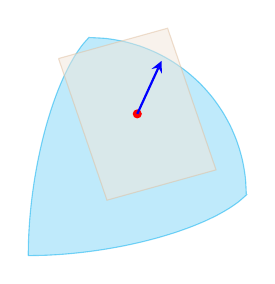
\begin{tikzpicture}[scale=0.5]
%% x^2+y^2+z^2 = 16, a level set of f(x,y,z) = x^2+y^2+z^2
%\drawxyz{4.5}
\draw[cyan,fill=cyan!50,opacity=0.5]
	plot[variable=\theta,domain=0:90, samples=15, smooth]
		(0,{4*sin(\theta)},{4*cos(\theta)})	--
	plot[variable=\theta,domain=0:90, samples=15, smooth]
		({4*sin(\theta)},{4*cos(\theta)},0)	--
	plot[variable=\theta,domain=0:90, samples=15, smooth]
		({4*cos(\theta)},0,{4*sin(\theta)});
%% draw tangent plane and normal at (2,2,2.83)
%% numerically the equation of the tangent plane is
%%	z=-0.707(x+y) + 5.65
%% bear in mind the usual scramble in tikz that (x,y,z) -> (y,z,x)
\draw[brown!50,fill=brown!20,opacity=0.5]	
	plot[variable=\t,domain=0:2, samples=15, smooth]
		({\t},{-0.707*(2+2*\t)+5.65}, {2+\t})
--
	plot[variable=\t,domain=0:2, samples=15, smooth]
		({2+\t},{-0.707*(6) + 5.65}, {4-\t})
--
	plot[variable=\t,domain=0:2, samples=15, smooth]
		({4-\t},{-0.707*(6-2*\t)+ 5.65},{2-\t})
--
	plot[variable=\t,domain=0:2, samples=15, smooth]
		({2-\t},{-0.707*2 + 5.65 },{\t});
\draw[red,fill=red]
	(2,2.83,2)	circle(0.1cm);
\draw[thick,blue,->,>=stealth]
	(2,2.83,2)	--	++(1,1.73,1);
\end{tikzpicture}
\end{textblock}

\end{frame}

%%%%%%%%%%%%%%%%%%%%%%%%%%%%%%%%%%%%%%%%%%%%%%%%%%%%%%
%%%%%%%%%%%%%%%%%%%%%%%%%%%%%%%%%%%%%%%%%%%%%%%%%%%%%%

\begin{frame}{Gradient - Examples}
\begin{textblock}{14.5}(1,3)
\begin{center}
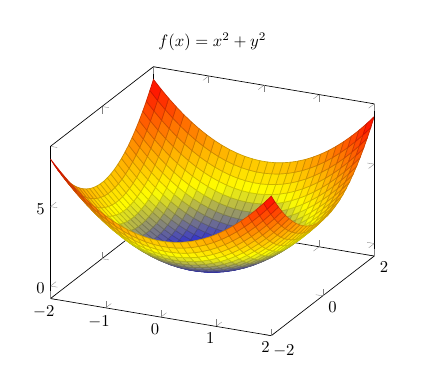
\begin{tikzpicture}[scale=0.6]
\begin{axis}
	[
		title={$f(x) = x^2+y^2$},
		domain=-2:2,
		axis background/.style={fill=white}
	]	
		\addplot3[surf,
			domain=-2:2,samples=30,z buffer=sort]
			{x^2+y^2};
\end{axis}
\end{tikzpicture}
\qquad
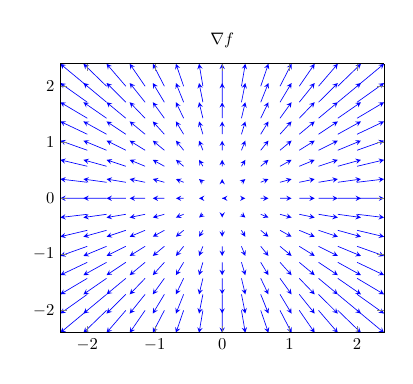
\begin{tikzpicture}[scale=0.6]
\begin{axis}
	[
		title={$\nabla f$},
		domain=-2:2,
		view={0}{90},
		axis background/.style={fill=white}
	]	
        \addplot3[blue,
            quiver={
             u={2*x},
             v={2*y},
             scale arrows=0.1,
            },
            -stealth,samples=15]
                {0};
\end{axis}
\end{tikzpicture}
\end{center}
\end{textblock}

\end{frame}

%%%%%%%%%%%%%%%%%%%%%%%%%%%%%%%%%%%%%%%%%%%%%%%%%%%%%%
%%%%%%%%%%%%%%%%%%%%%%%%%%%%%%%%%%%%%%%%%%%%%%%%%%%%%%

\begin{frame}{Gradient - Examples}
\begin{textblock}{6}(1,3)

\begin{itemize}

	\item Find the gradient of $f(x,y,z) = x^4 + y^4$
	
	\item Find the gradient of $f(x,y,z) = xy$ at the point (-4,5)

\end{itemize}

\end{textblock}
\end{frame}


%%%%%%%%%%%%%%%%%%%%%%%%%%%%%%%%%%%%%%%%%%%%%%%%%%%%%%
%%%%%%%%%%%%%%%%%%%%%%%%%%%%%%%%%%%%%%%%%%%%%%%%%%%%%%

\begin{frame}{Curl}
\begin{textblock}{14.5}(1,3)
\begin{myblock}[0.8]{}

\eq{
\curl F = 
	\begin{vmatrix}
	\dfrac{\hat{u_1}}{h_2 h_3}  & \dfrac{\hat{u_2}}{h_1 h_3} & \dfrac{\hat{u_3}}{h_1 h_2} \\[12pt]
	\partd{}{u_1} & \partd{}{u_2} & \partd{}{u_3} \\[12pt]
	h_1 F_1 & h_2 F_2 & h_3 F_3 
	\end{vmatrix}
}

\end{myblock}
\end{textblock}

\end{frame}

%%%%%%%%%%%%%%%%%%%%%%%%%%%%%%%%%%%%%%%%%%%%%%%%%%%%%%
%%%%%%%%%%%%%%%%%%%%%%%%%%%%%%%%%%%%%%%%%%%%%%%%%%%%%%

\begin{frame}{Curl - Examples}
\begin{textblock}{14.5}(1,3.5)
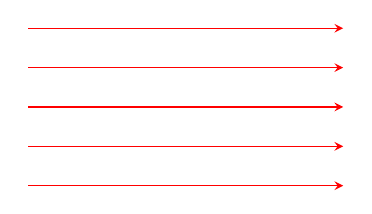
\begin{tikzpicture}[scale=2]
\foreach\y in {0,0.25,...,1}{
	\draw[-stealth, red] (0,\y) -- (2,\y);
}
\end{tikzpicture}%

\vspace{18pt}

\begin{tikzpicture}[scale=2]
\foreach\x/\y in {0.25/0.25,0.5/0.5,0.75/0.75,1/1}{
	\draw[-stealth] (0,\y) -- (\x,\y);
}
\end{tikzpicture}

\vspace{18pt}


\begin{tikzpicture}[scale=1.25]
\foreach\r in {0.25, 0.5,...,1}{
	\draw[decoration={markings, mark=at position 0.625 with {\arrow{>}}},
        postaction={decorate}] (0,0) circle (\r); 
}
\end{tikzpicture}
\end{textblock}

\begin{textblock}{7}(8,3)
Determine the rotation in the field:
\eq{
	\vec{H} = \xhat\lp 3y + \dfrac{z^2}{2}\rp +\yhat\lp 2x-z\rp + \zhat 3xy
}
\end{textblock}
\end{frame}

%%%%%%%%%%%%%%%%%%%%%%%%%%%%%%%%%%%%%%%%%%%%%%%%%%%%%%
%%%%%%%%%%%%%%%%%%%%%%%%%%%%%%%%%%%%%%%%%%%%%%%%%%%%%%

\begin{frame}{Divergence}
\begin{textblock}{14.5}(1,3)
\begin{myblock}[0.9]{}

\eq{
	\nabla\mycdot f = \dfrac{1}{h_1 h_2 h_3} \lb \dfrac{1}{h_1}\partd{h_2 h_3 f_1}{u_1} + \dfrac{1}{h_2}\partd{h_1 h_3 f_2}{u_2} + \dfrac{1}{h_3}\partd{h_1 h_2 f_3}{u_3} \rb
}

\end{myblock}

\end{textblock}

\end{frame}

%%%%%%%%%%%%%%%%%%%%%%%%%%%%%%%%%%%%%%%%%%%%%%%%%%%%%%
%%%%%%%%%%%%%%%%%%%%%%%%%%%%%%%%%%%%%%%%%%%%%%%%%%%%%%

\begin{frame}{Divergence - Example}
\begin{textblock}{14.5}(1,3.5)
Determine the electric flux through a point $(x, y, z)$ of the field:
\eq{
	\vec{H} = \xhat \lp 3y + \dfrac{z^2}{2} \rp + \yhat\lp 2x-z\rp + \zhat 3xy
}
\end{textblock}

\end{frame}

%%%%%%%%%%%%%%%%%%%%%%%%%%%%%%%%%%%%%%%%%%%%%%%%%%%%%%
%%%%%%%%%%%%%%%%%%%%%%%%%%%%%%%%%%%%%%%%%%%%%%%%%%%%%%

\begin{frame}{What is Divergence, really?}
\begin{textblock}{14.5}(1,3.5)
\begin{itemize}
	\item Amount of a field ``leaving'' an enclosed surface:
	\vspace{-8pt}
	\eq{
		\nabla \mycdot \vec{F} = \lim_{\Delta v \to 0} \dfrac{\oiint\limits_{S}	\vec{F}\mycdot d\vec{S}}{\Delta v}
	}
	\item Gauss' Law:
		\vspace{-8pt}
	\eq{
		\oiint\limits_{S} \vec{D} \mycdot d\vec{S} 
		=\oiint\limits_{S} \epsilon\vec{E} \mycdot d\vec{S} 
		= Q_{\text{enclosed}} \qquad\text{and}\qquad
		\nabla \mycdot \vec{D} = \rho_v
	}
	
\end{itemize}
	\vspace{-18pt}

\end{textblock}

\end{frame}

%%%%%%%%%%%%%%%%%%%%%%%%%%%%%%%%%%%%%%%%%%%%%%%%%%%%%%
%%%%%%%%%%%%%%%%%%%%%%%%%%%%%%%%%%%%%%%%%%%%%%%%%%%%%%

\begin{frame}{Laplacian}
\begin{textblock}{14.5}(1,3.5)

\eq{
	&\nabla^2 V(x,y,z) = \partd{^2 V}{x^2} + \partd{^2 V}{y^2} + \partd{^2 V}{z^2} \\
	&\nabla^2 V(\rho,\phi,z) = \dfrac{1}{\rho}\partd{}{\rho}\lp\rho\partd{V}{\rho}\rp + \dfrac{1}{\rho^2}\partd{^2 V}{\phi^2} + \partd{^2 V}{z^2} \\
	&\nabla^2 V(r,\theta,\phi) = \dfrac{1}{r^2}\partd{}{r}\lp r^2 \partd{ V}{r}\rp \\
	&+ \dfrac{1}{r^2 \sin{\theta}}\partd{}{\theta}\lp\sin{\theta}\partd{V}{\theta}\rp + \dfrac{1}{r^2\sin{\theta}^2}\partd{^2 V}{\phi^2} \\	
}
\end{textblock}

\end{frame}


%%%%%%%%%%%%%%%%%%%%%%%%%%%%%%%%%%%%%%%%%%%%%%%%%%%%%%
%%%%%%%%%%%%%%%%%%%%%%%%%%%%%%%%%%%%%%%%%%%%%%%%%%%%%%

\begin{frame}{Laplacian Examples}
\begin{textblock}{14.5}(1,3.5)

\begin{itemize}
	\def\itemsep{18pt}
	\item Find the Laplacian of $f(x,y,z) = e^{xyz}$
	
	\item Find the Laplacian of $f(x,y,z) = \dfrac{1}{x^2 + y^2 + z^2}$
\end{itemize}

\end{textblock}

\end{frame}

%%%%%%%%%%%%%%%%%%%%%%%%%%%%%%%%%%%%%%%%%%%%%%%%%%%%%%
%%%%%%%%%%%%%%%%%%%%%%%%%%%%%%%%%%%%%%%%%%%%%%%%%%%%%%

\begin{frame}{Divergence Theorem \& Stoke's Theorem}
\begin{textblock}{14.5}(1,3.5)

\begin{myblock}[0.9]{Divergence Theorem}
	\eq{
		\iiint\limits_V \nabla\mycdot \vec{D} dV 
		= \oiint\limits_S \vec{D}\mycdot d\vec{S}
	}
\end{myblock}


\begin{myblock}[0.9]{Stoke's Theorem}

\center\eq{
	\iint_S \lp\nabla\times F \rp\mycdot dS = \oint_C F\mycdot d\ell
}

\end{myblock}


\end{textblock}

\end{frame}


%%%%%%%%%%%%%%%%%%%%%%%%%%%%%%%%%%%%%%%%%%%%%%%%%%%%%%
%%%%%%%%%%%%%%%%%%%%%%%%%%%%%%%%%%%%%%%%%%%%%%%%%%%%%%

\begin{frame}{Stoke's Theorem}
\begin{textblock}{14.5}(0.5,3.5)
Verify the contour integral, using Stoke's theorem:

$\vec{E} = \hat{\rho} \rho \sin{\phi} + \hat{\phi} \rho^2$ over the contour $(0,0,0) - (2,0,0) - (2,\dfrac{\pi}{2},0) - (0,\dfrac{\pi}{2},0)$
\end{textblock}
\end{frame}









